\documentclass[12pt,letterpaper,titlepage]{article}

\usepackage{fontspec}
\defaultfontfeatures{Mapping=tex-text}
\usepackage{xunicode}
\usepackage{xltxtra}
\usepackage{amsmath}
\usepackage{pdfpages}
\usepackage{amsfonts}
\usepackage{bbold}
\usepackage{amssymb}
\setcounter{secnumdepth}{0}
\usepackage{nameref}
\usepackage{enumitem}
\usepackage{environ}
\usepackage{pgfplots}

\showboxdepth=\maxdimen
\showboxbreadth=\maxdimen


\usepackage{paracol}
\usepackage{wrapfig}
\globalcounter{table}
\globalcounter{figure}
\usepackage{graphicx}
\usepackage[left=1in,right=1in,top=1in,bottom=1in]{geometry}
\graphicspath{{img/}}

\author{Jacob Abel}
\title{	Exam 1 Proposed Problems
	\\\large ECE2204 CRN:82929
}

\setlength{\parskip}{0.5em}

\begin{document}
\maketitle
\begin{raggedright}

\section{Problem 1: } Derived from p1.17 by changing values and swapping $D_p$ and $J_p$.
\subsection{Design}
The hole concentration in silicon is given by 

\begin{equation}\scalebox{1.25}{
$
p(x) = 10^3 + 10^{12} e^\frac{−x}{L_p}\quad x \geq 0
$
}
\end{equation}

The value of $L_p$ is $13\mu m$. The hole diffusion current density is $J_p = 1.44 \times 10^{-3} A/cm^2$. Assume the value of the elementary charge is $\mathbb{e} = 1.6\cdot 10^{-19} C$. Determine the hole diffusion current density at $x = 23\mu m$.

\begin{equation}\scalebox{1.25}{
$
\frac{dp}{dx}p(x) = \frac{-10^{12}}{L_p} e^\frac{-x}{L_p}
$
}
\end{equation}

\begin{equation}\scalebox{1.25}{
$
J_p = -\mathbb{e} D_p \frac{dp}{dx} \implies D_p = \frac{L_p\times J_p \times e^\frac{x}{L_p} \times cm^{3}}{\mathbb{e}\times 10^{12} }
$
}
\end{equation}

\begin{equation}\scalebox{1.25}{
$
J_p = \frac{13\mu m\times 1.44 \times 10^{-3} A/cm^2\times e^\frac{23\mu m}{13\mu m} \times cm^{3}}{1.6\times 10^{-19} C\times 10^{12}}
	= 68.64 cm^2/s
$
}
\end{equation}



The hole diffusion coefficient is $D_p = 68.64 cm^2/s$.

\subsection{Validation}

\begin{center}
LTSpice Implementation (accurate with $< 1\%$ deviation from design result)
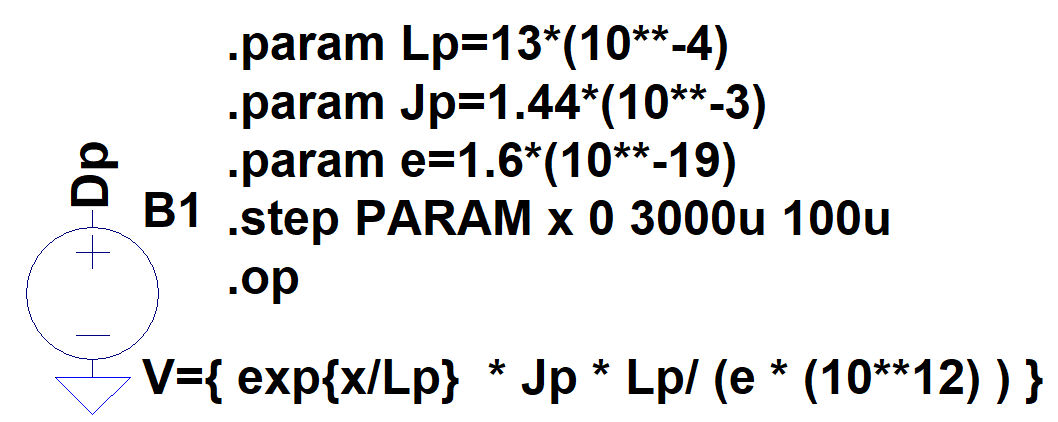
\includegraphics[width=.4\textwidth, height=\textheight, keepaspectratio=true]{ds2b}
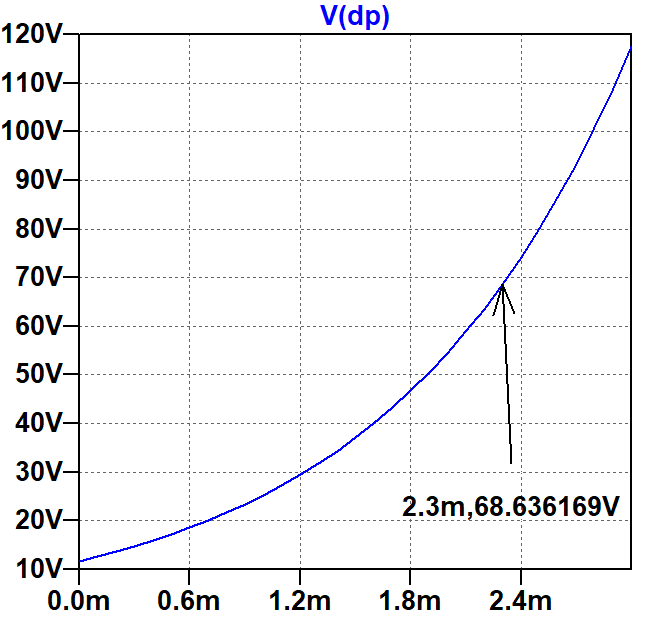
\includegraphics[width=.4\textwidth, height=\textheight, keepaspectratio=true]{ds2c}
$Err = \frac{|68.64-68.636|}{68.64} = 0.00005 = 0.01\%$
\end{center}
\clearpage

\section{Problem 2: } What is the variable $I_S$, what is its unit, what happens when $I_S$ increases or decreases?

$I_S$ is the reverse bias saturation current. As it is a current, it has a unit of Amperes. This variable is one of the major drivers of the ideal pn junction current-voltage equation. Therefore increasing $i_d$ is directly dependent on $I_S$.

\end{raggedright}
\end{document}
